\section{Résultats}

\subsection{Présentation des rendus}

\begin{figure}[H]
    \centering
    \begin{minipage}[t]{0.48\textwidth}
        \centering
        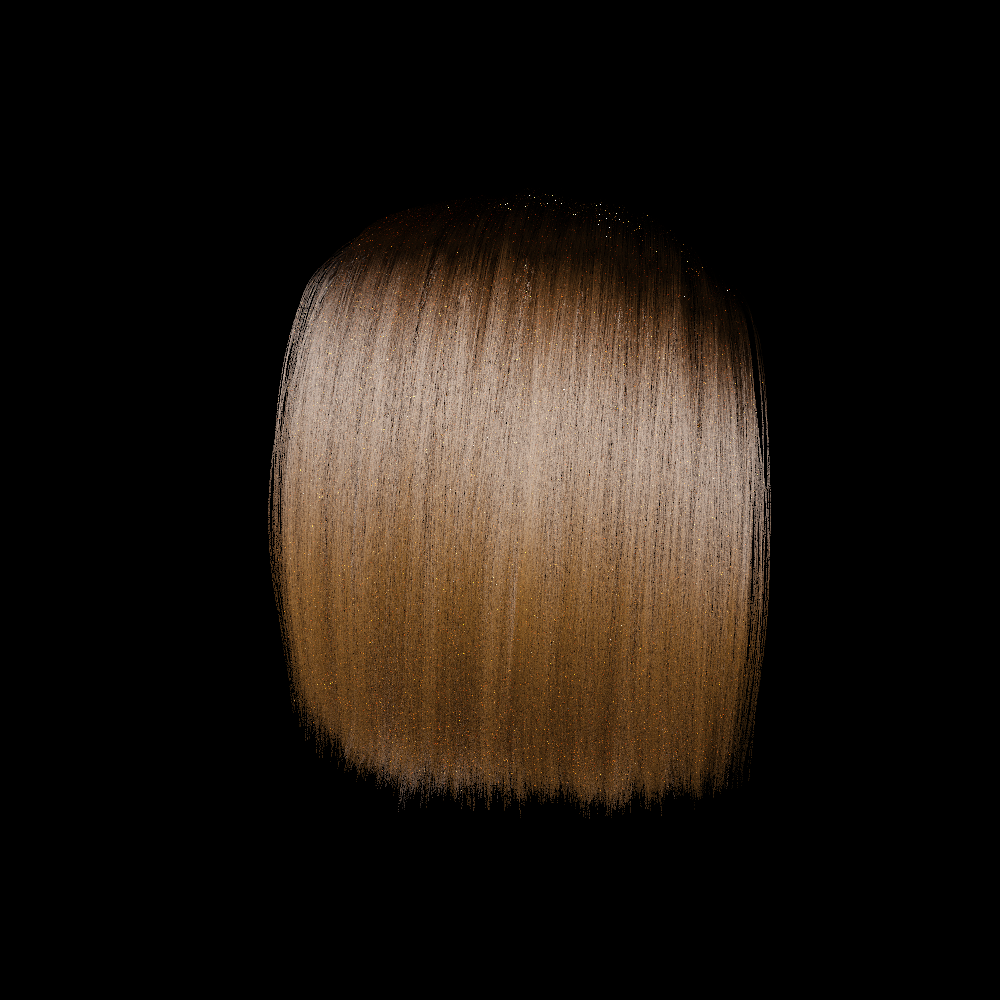
\includegraphics[width=\textwidth]{figures/img-validation.png}
        \caption{Image de validation : rendu de référence avec Embree.}
        \label{fig:img-validation}
    \end{minipage}
    \hfill
    \begin{minipage}[t]{0.48\textwidth}
        \centering
        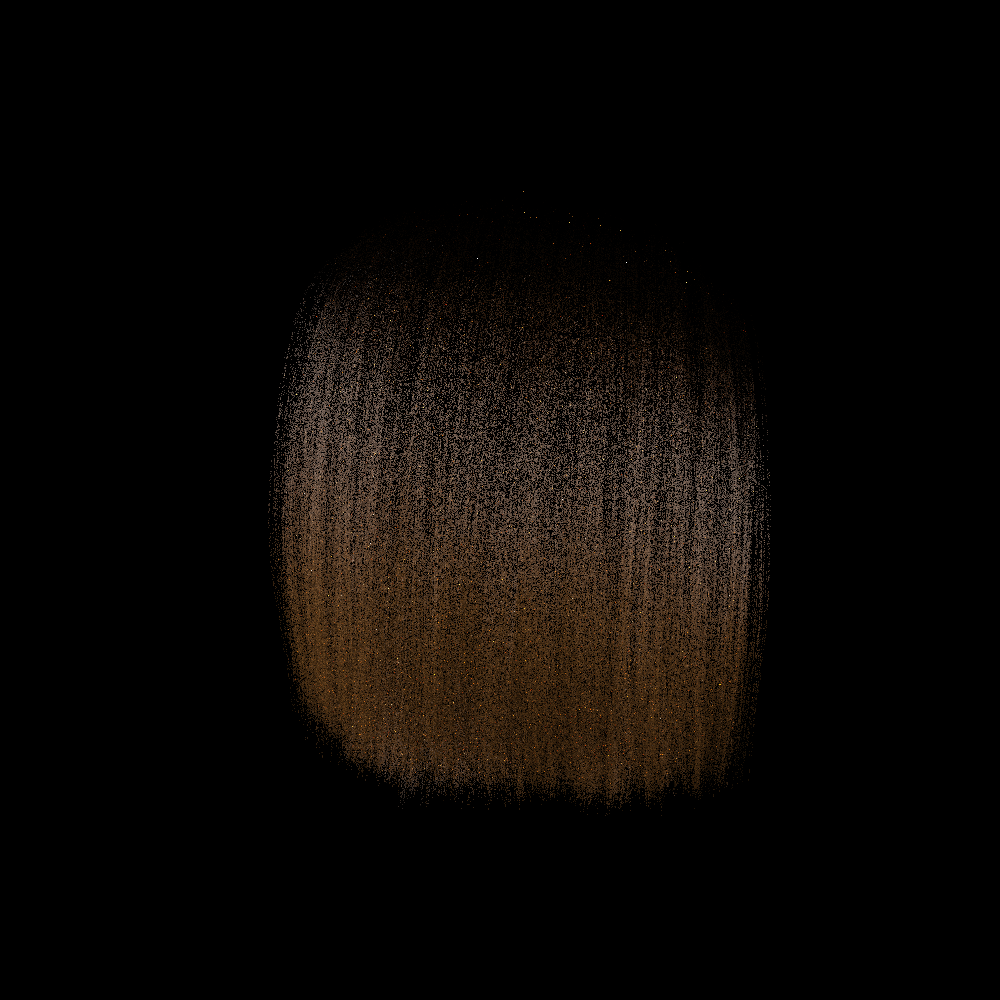
\includegraphics[width=\textwidth]{figures/profile_gpis_amp_0_4.png}
        \caption{Rendu utilisant la technique GPIS.}
        \label{fig:gpis_render}
    \end{minipage}
\end{figure}

La figure~\ref{fig:img-validation} est un rendu avec la géométrie d'Embree pour les courbes qui servira d'image de référence pour la validation, et la figure~\ref{fig:gpis_render} est un rendu avec la technique GPIS. Les deux utilisent le modèle de réflexion de \textcite{deon2011egsr} ; on remarque que l'image de droite a une réflexion moins prononcée, due au fait que les normales sont tirées du processus stochastique. En observant le contour du modèle, on observe la disparition spontanée de certains cheveux, qui cause l'apparence vaporeuse des GPIS.

\begin{figure}[H]
    \centering
    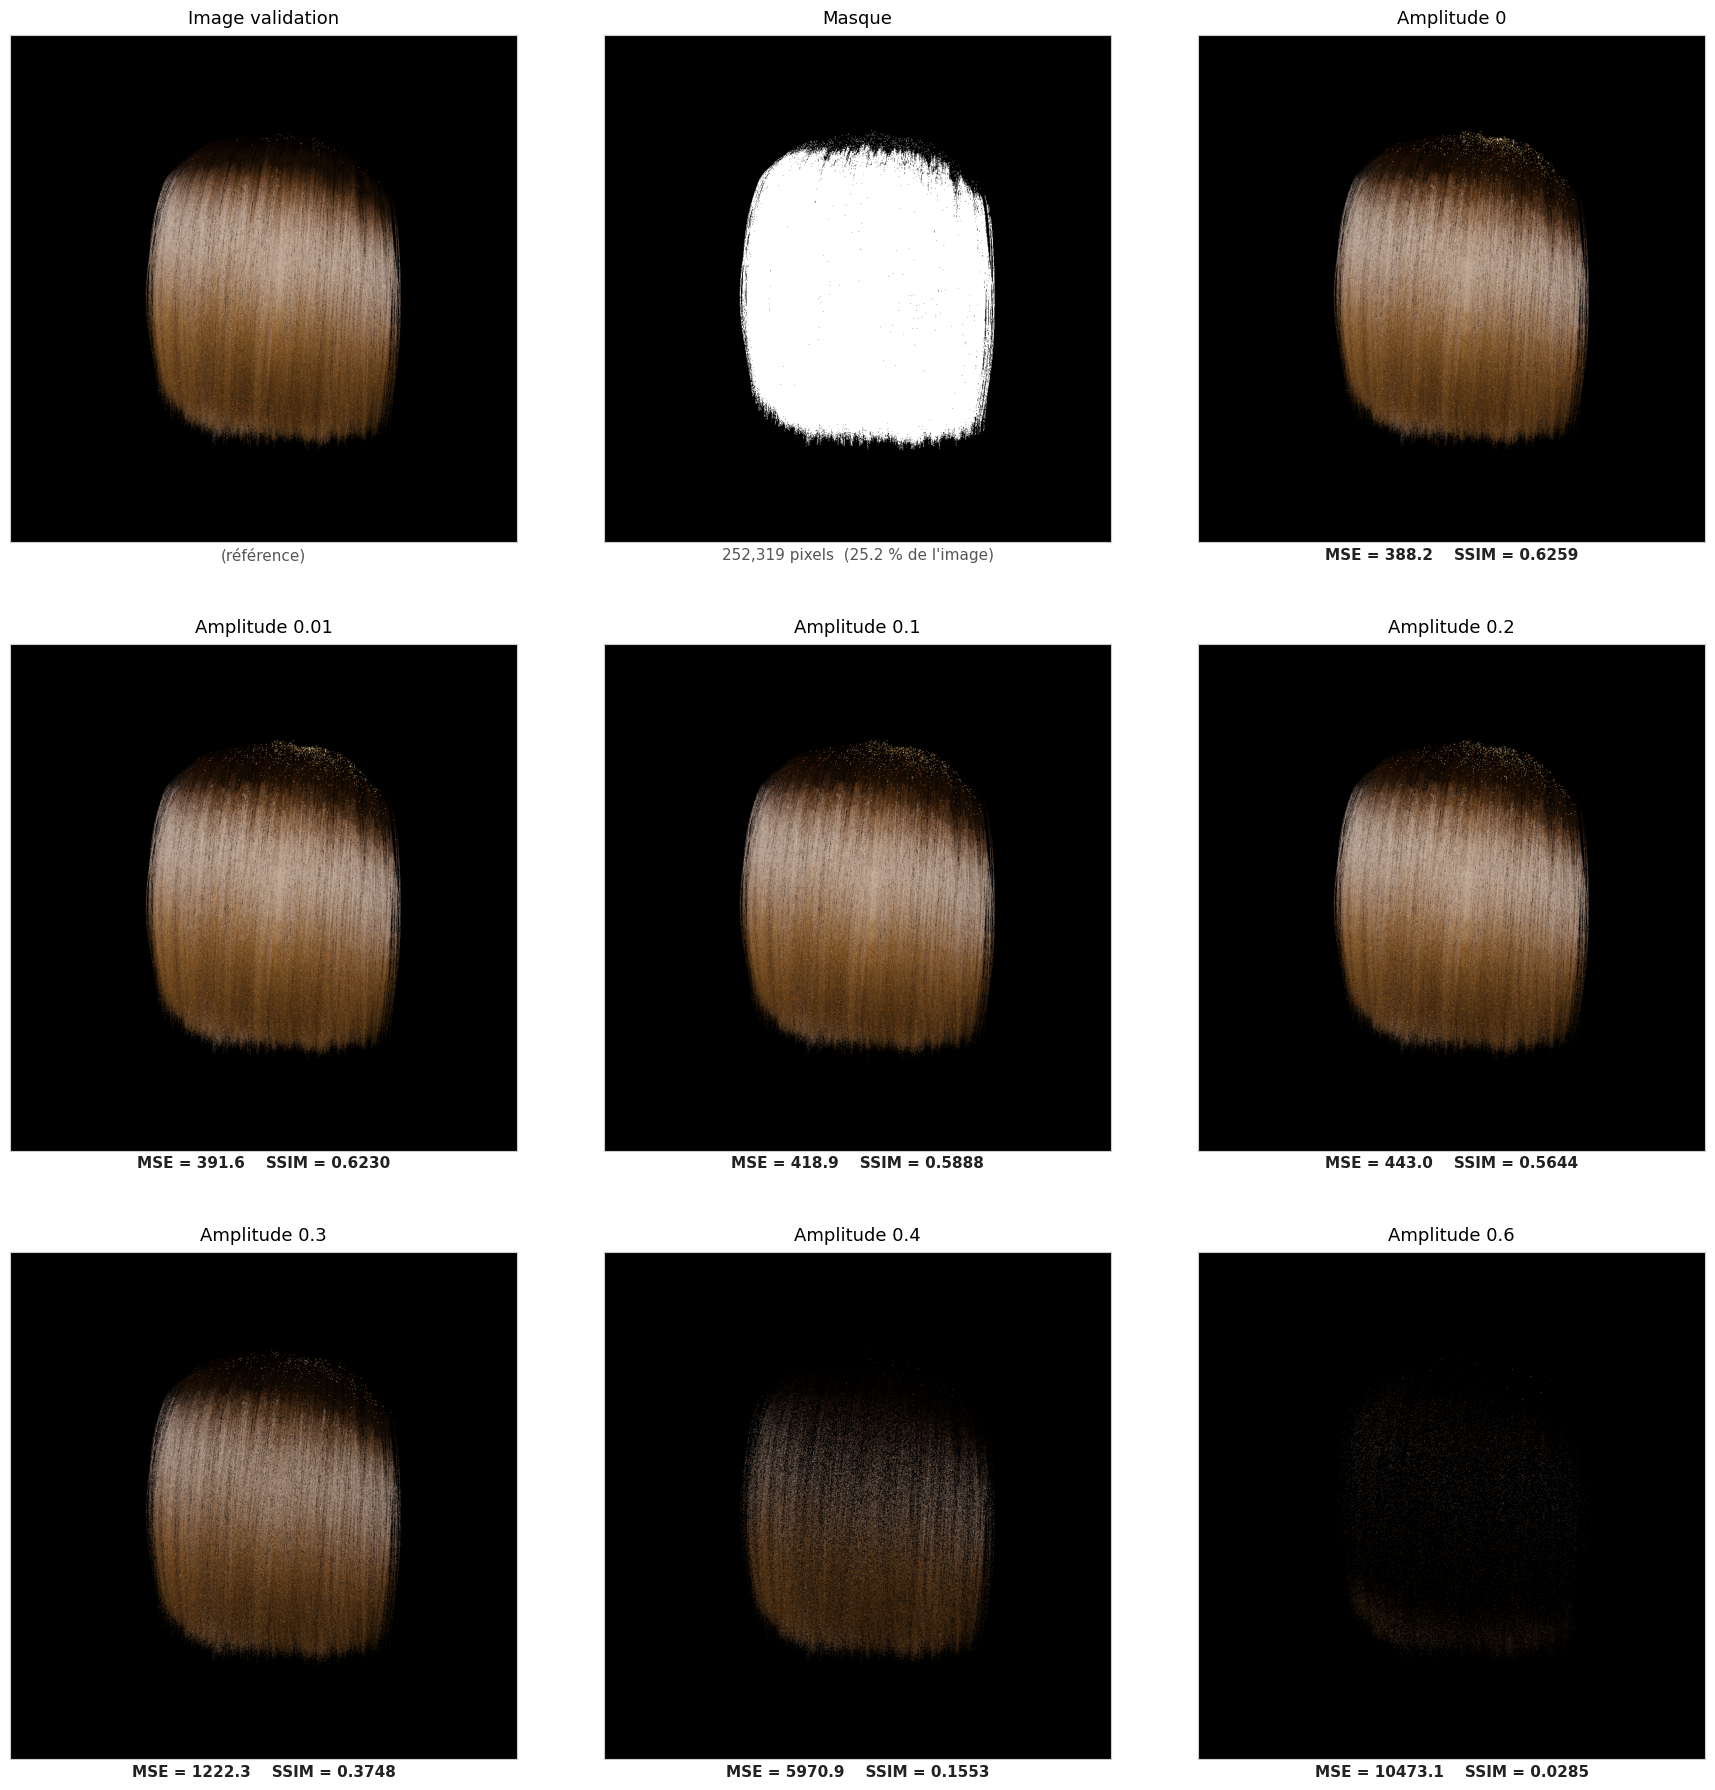
\includegraphics[width=\textwidth]{figures/comparaison-9x9.png}
    \caption{Comparaison des rendus GPIS par rapport à l'image de validation pour sept niveaux d'amplitude de covariance.}
    \label{fig:comparaison-9x9}
\end{figure}

Le tableau~\ref{fig:comparaison-9x9} présente une comparaison entre les rendus GPIS et l'image de vérification en calculant l'erreur quadratique moyenne (MSE) à partir de la distance euclidienne des valeurs RGB, et la mesure de similarité structurelle (SSIM) entre chaque image et l'image de vérification. Afin de retirer le fond noir de l'image dans l'équation, les valeurs de SSIM et de MSE sont calculées uniquement sur une région masquée définie par les pixels non noirs sur l'image de référence. Une valeur de 0 pour la MSE signifie des images identiques, et une valeur de 1,0 pour la SSIM signifie deux images identiques.

\begin{figure}[H]
    \centering
    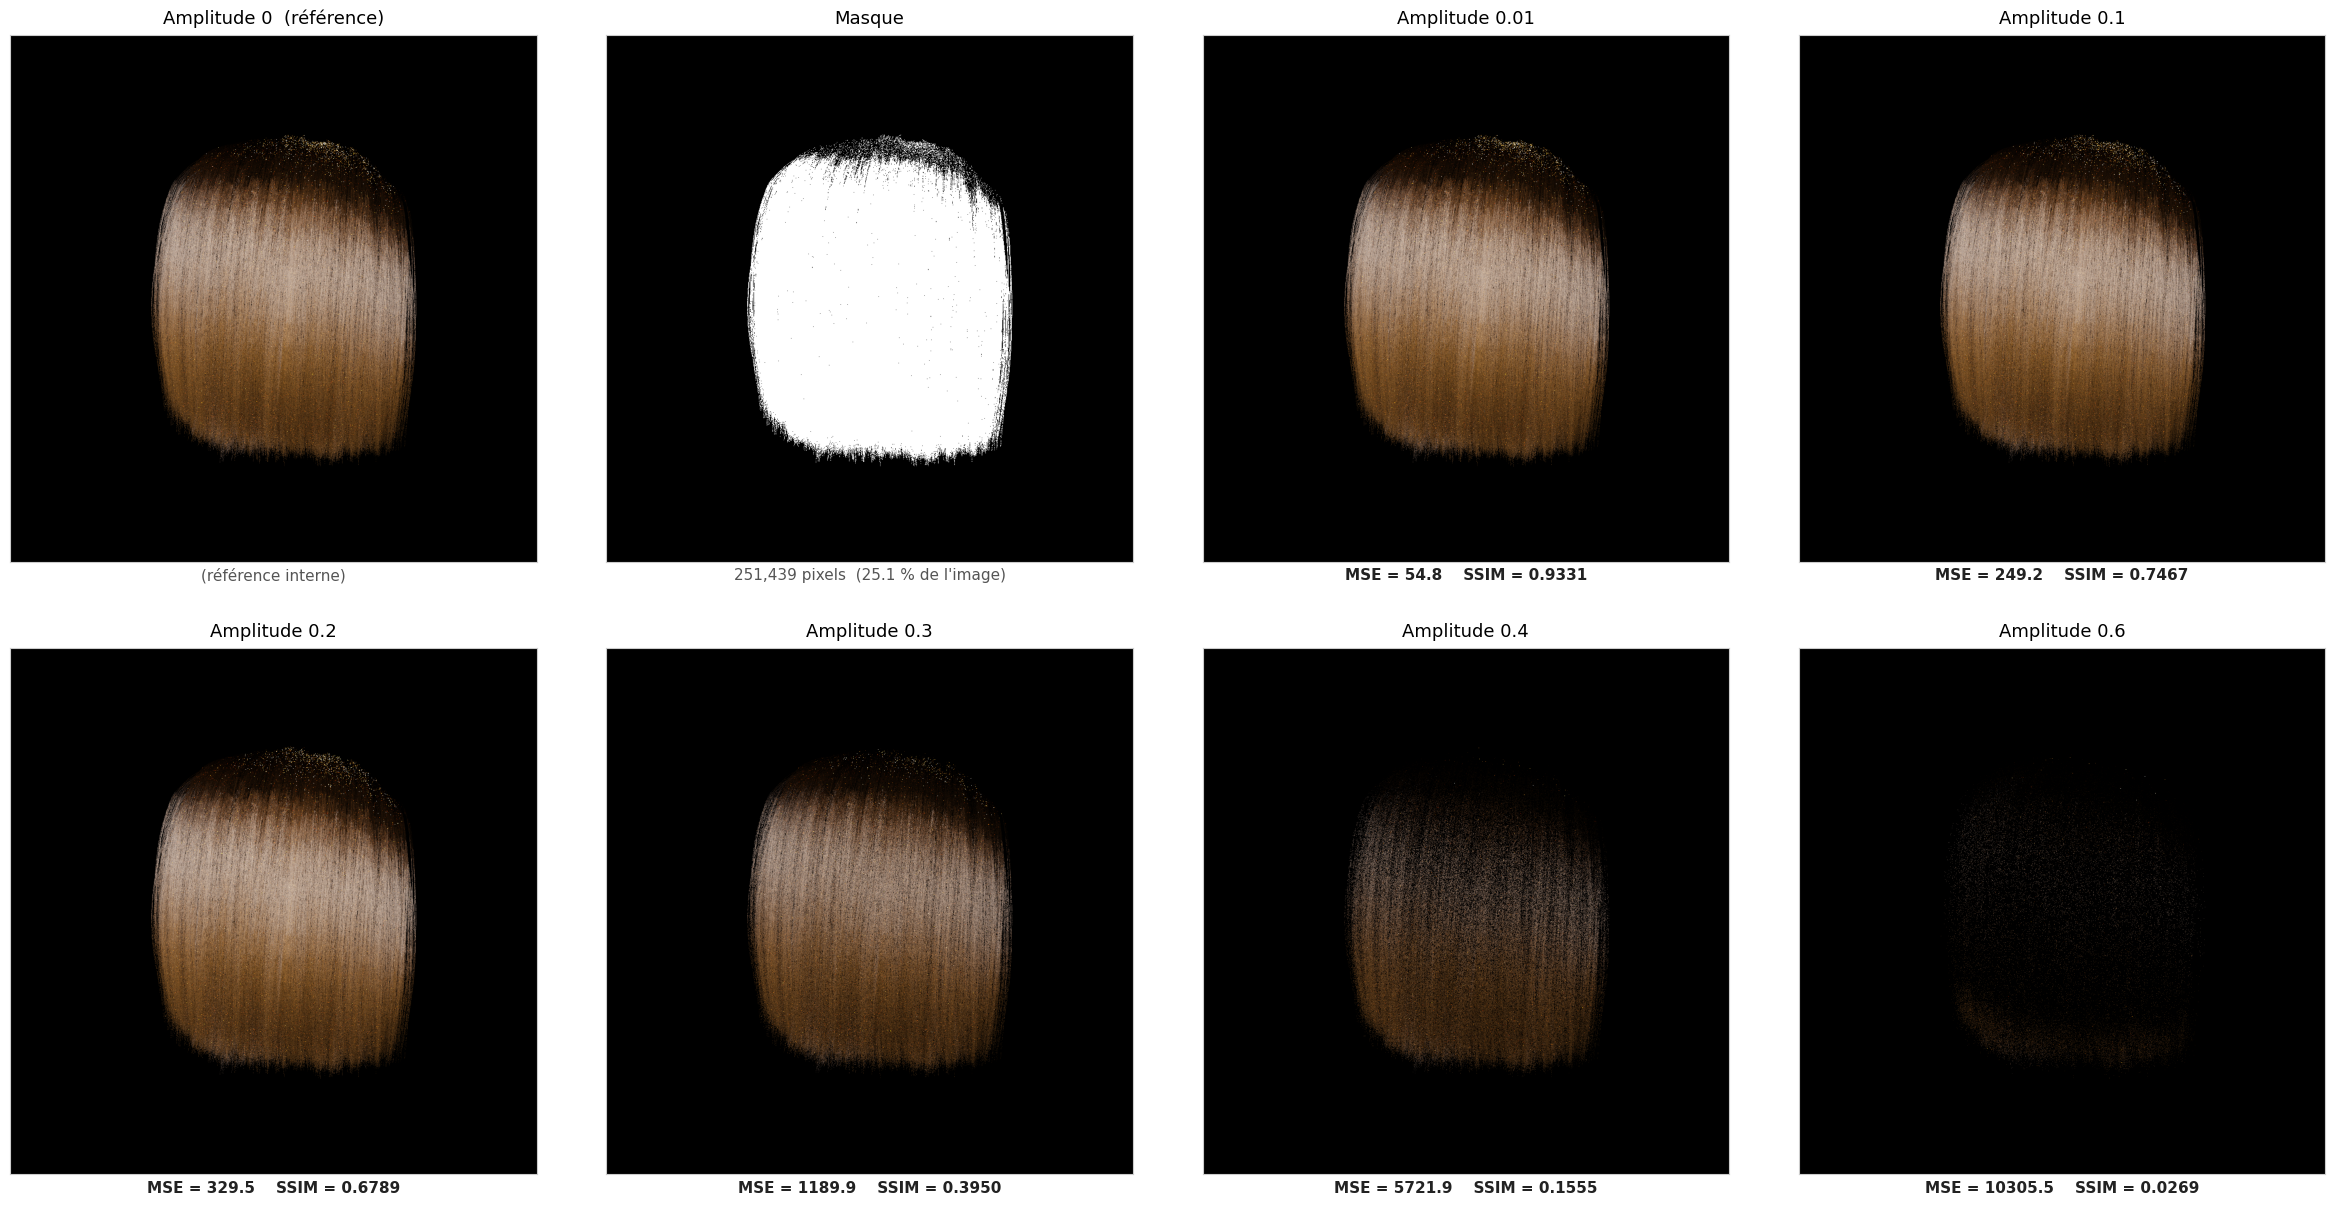
\includegraphics[width=\textwidth]{figures/comparaison-2x4.png}
    \caption{Comparaison des rendus GPIS entre eux, en utilisant le rendu à 0 amplitude comme image de référence.}
    \label{fig:comparaison-2x4}
\end{figure}

Le tableau~\ref{fig:comparaison-2x4} présente une comparaison entre les rendus GPIS en utilisant le rendu avec 0 amplitude comme image de validation. On compare les MSE et les SSIM des différents rendus.

Tous les rendus sont effectués sur un ordinateur Dell OptiPlex 5080 avec un processeur Intel Core i5-10500 @ 3,10~GHz, 6 coeurs et 12 fils d'exécution.

\subsection{Analyse}

L'image utilisée comme image de vérification est la figure~\ref{fig:img-validation}. Le modèle de cheveux contient 1 million de courbes représentées par 4 points 3D dans l'espace. Le rendu est effectué à partir du tracé de rayon développé avec Embree ; pour trouver l'emplacement de la surface, une approche déterministe est utilisée puisque Embree supporte déjà les courbes. Le rendu est effectué pour une résolution de 1000$\times$1000 pixels. Le moteur de rendu lance 16 rayons par pixel. La couleur, la réfraction et la réflexion sur les cheveux sont calculées avec le modèle de \textcite{deon2011egsr}, que j'ai implémenté dans le moteur.

\subsubsection{Effet de l'amplitude de la covariance}

J'ai introduit un facteur d'amplitude de la covariance dans l'échantillonnage (équation~\ref{eq:echantillonnage}) de la surface, qui permet de modifier l'impact de la covariance sur la moyenne :
\[
f(\mathbf{x}) = \mu(\mathbf{x}) + a \cdot \sigma
\]
Les tableaux~\ref{fig:comparaison-9x9} et~\ref{fig:comparaison-2x4} présentent 7 niveaux d'amplitude de la covariance : 0,0 ; 0,01 ; 0,1 ; 0,2 ; 0,3 ; 0,4 et 0,6. À 0,0, la covariance du processus est ignorée et seule la moyenne est utilisée pour trouver l'intersection.

On réalise qu'en augmentant l'impact de la covariance, l'algorithme n'arrive plus à détecter une intersection avec la surface du cheveu. En effet, le rayon ne peut plus détecter la surface puisqu'elle tend à se déplacer vers une distance infiniment petite, causant le tracé de rayon à ne pas détecter la surface lors du \textit{raymarching}. On remarque qu'à 0,4, on obtient l'apparence vaporeuse désirée, rappelant ce que l'on observe dans les rendus de \textcite{seyb24from} (figure~\ref{fig:seyb24-teaser}) ; c'est d'ailleurs cette amplitude qui est utilisée pour la figure~\ref{fig:gpis_render}.

\subsubsection{Comparaison qualitative}

Les rendus GPIS, même avec une amplitude nulle, ont une réflexion moins prononcée que l'image de validation (figure~\ref{fig:img-validation}). Cela est dû au fait que les normales sont tirées du processus stochastique dans tous les cas, ce qui les rend plus chaotiques et forme ainsi des reflets moins uniformes.

Dans le rendu de validation, mais surtout pour le rendu à 0 amplitude, des lucioles très apparentes sur le dessus et le bas des cheveux constituent un effet non désiré lié à un algorithme de tracé de rayon immature. Ce sont des pixels trop illuminés comparés à leurs voisins. Cet effet est causé par des rayons qui passent à un angle rasant près des courbes. En effet, la détection de collision avec la surface utilise une petite constante $\varepsilon$ pour détecter la collision, ce qui déclenche la collision alors que le rayon est rasant sur la courbe et ne serait pas supposé toucher. On comprend donc que la technique de \textit{raymarching} implémentée produit implicitement des différences avec l'approche optimale d'Embree.

\subsubsection{Comparaison quantitative}

Les valeurs élevées de MSE, particulièrement pour les rendus à basse amplitude (388 pour le rendu à 0 amplitude et 391 pour le rendu à 0,01 amplitude, où on s'attend à obtenir un rendu presque identique), sont majoritairement dues aux lucioles : un pixel avec une grande distance entre la couleur attendue et la couleur obtenue peut rapidement faire augmenter l'erreur d'un rendu qui est visuellement similaire. L'utilité du SSIM est de limiter la contribution de ces facteurs ; on obtient tout de même des valeurs basses d'environ 62~\% pour les deux, ce qui est dû à la réflexion moins prononcée expliquée par les normales stochastiques. Pour les autres rendus, les valeurs de MSE et de SSIM se dégradent comme attendu lorsqu'on s'éloigne d'une représentation fidèle vers une représentation plus vaporeuse.

La comparaison dans la figure~\ref{fig:comparaison-2x4} avec l'image à 0 amplitude permet de comparer les rendus GPIS entre eux, permettant ainsi de constater que les images qui devraient avoir une grande ressemblance, comme l'amplitude 0 et l'amplitude 0,01, conservent 93~\% de similarité structurelle, avec une similarité qui se dégrade progressivement jusqu'à atteindre 2~\% pour le rendu avec une amplitude de 0,6, où la chevelure est pratiquement disparue. Les MSE commencent avec une petite valeur de 54 entre 0 et 0,01, suivie de valeurs d'erreur qui croissent rapidement avec la dégradation de l'image.

\subsection{Temps de rendu}

L'image de validation prend en moyenne 120 secondes à rendre pour une image 1000$\times$1000 à 16 rayons par pixel. Pour des paramètres identiques, une image GPIS prend en moyenne 25\,000 secondes à rendre (environ 7h). Cet écart est dû non seulement au temps de calcul de l'approximation du processus gaussien, mais aussi au coût implicite de l'algorithme de \textit{raymarching}, qui évalue plusieurs points le long du rayon comparé à un algorithme de tracé de rayon qui trouve analytiquement le point d'intersection avec une surface. La preuve en est que le calcul de l'image avec 0 amplitude (où le calcul de la variance est ignoré) prend quand même 500 secondes.

Un facteur non trivial est la température du CPU sur le banc de test. En effet, puisque le programme utilise tous les coeurs du CPU, il a tendance à faire monter rapidement la température de l'ordinateur. En réponse, le micrologiciel de l'ordinateur réduit la fréquence du processeur. Cela a un impact lors du banc de test puisque les rendus sont effectués les uns après les autres sans rétablir la température du CPU, mais aussi lors d'un seul rendu : le CPU sera beaucoup plus chaud vers la fin, ce qui ralentit le rendu.
